\begin{appendices}
\section{Sequential Algorithms}\label{app:algorithms}
The progressive optimization of matrix multiplication relies heavily on understanding how modern hardware manages memory. This section details the theoretical and practical logic behind the sequential algorithms evaluated, illustrating the shift from a direct mathematical translation to a highly optimized, hardware-aware implementation.


\subsection{Naive Approach: $i-j-k$}\label{subsec:ijk}

The standard triple-nested loop represents the most intuitive translation of the mathematical definition of matrix multiplication. For square matrices A and B, the product matrix C is defined as:

$$C_{ij}=\sum_{k=1}^{n}A_{ik}\cdot B_{kj}$$

To compute a single element $C_{ij}$, the algorithm calculates the complete dot product between the $i$-th row of matrix A and the $j$-th column of matrix B. 
While mathematically sound, this approach is highly inefficient for large matrices: because the innermost loop iterates over $k$, the algorithm accesses the elements of $B_{kj}$ by jumping across distinct rows in memory. 

In standard C-style row-major memory layouts, this column-wise traversal breaks the \emph{spatial locality} exploited by the caching: it forces the CPU to continuously fetch new cache lines from main memory, leading to poor cache utilization and significant execution stalls.

Note that this implementation performs so badly that it is not even cited in this report, that starts directlyu with  the next approach

\subsection{Standard Approach: $i-k-j$}\label{subsec:ikj}

To address the severe memory inefficiencies of the naive implementation, the standard optimization involves a simple structural adjustment: swapping the order of the inner loops to $i-k-j$. Reordering the loops fundamentally changes the sequence of the arithmetic operations without altering the final mathematical result. Instead of calculating a single element $C_{ij}$ to completion, this approach takes a scalar element $A_{ik}$ and multiplies it across the entire $k$-th row of B, accumulating those partial results into the $i$-th row of C.

The innermost loop executes as follows:
\begin{verbatim}
for (int j = 0; j < n; j++)
    C[i][j] += A[i][k] * B[k][j];
\end{verbatim}

By making $j$ the innermost loop, the algorithm ensures that both matrix C and matrix B are accessed in a linear fashion: as $j$ increments, the memory addresses requested are strictly sequential. 

This continuous row-major traversal takes full advantage of spatial locality and hardware prefetching mechanisms, keeping the CPU pipelines fed and drastically reducing overall memory latency.

\subsection{Better Approach: Tiling (Blocking)}\label{subsec:tiling}


While the $i-k-j$ approach successfully linearizes access, its performance degrades when the active working set exceeds the capacity of the CPU's cache hierarchy. If the matrices are large enough, an entire row may be evicted from the cache before the algorithm can return to reuse it in the next iteration. Loop tiling (also known as blocking) directly addresses this limitation.

\begin{figure}[H]
    \centering
    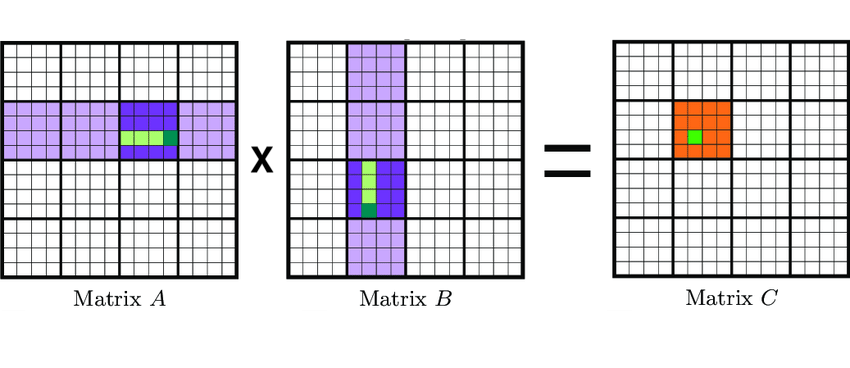
\includegraphics[width=0.8\linewidth]{appendices/tiling.png}
    \caption{Loop decomposition to allow for Explicit Tiling}
    \label{fig:tiling_image}
\end{figure}

Tiling decomposes the standard n-depth loop nest into a more complex, deeply nested structure : it partitions the vast iteration space into smaller, fixed-size geometric blocks, or tiles. By restricting the active computation to a specific tile, the compiler effectively limits the kernel's active working set. 

This methodology prevents the \textbf{cache thrashing} typical of naive matrix multiplication, where data is evicted before it can be reused in the next outer-loop iteration. Because the data blocks remain resident in the cache for the duration of the tile's computation, the algorithm maximizes temporal locality and avoids the massive latency penalty of repeatedly fetching data from main memory.

This implementation can be exploited by the compiler in a autonomous way, as  we have addressed in Subsection~\ref{subsec:seq_3}; nonetheless the explicit partitioning in "working sets" still suffer from the \emph{cache-associativity} problem, hence it requires further optimizations.

\subsection{Best implementation: \texttt{OpenBlas} }\label{subsec:openblas}

While standard loop tiling ensures that active matrix blocks fit within the CPU's cache, it does not solve the fundamental issue of memory continuity. Because the original matrices $A$ and $B$ are allocated in a standard row-major layout, a two-dimensional tile extracted directly from them still consists of fragmented memory segments: jumping across these non-contiguous rows inside the cache can trigger associative cache collisions and memory stalls. 

To approach peak theoretical hardware limits, we must abandon in-place computation and adopt explicit data packing strategies characteristic of the OpenBLAS/BLIS architecture.

\begin{figure}[H]
\centering
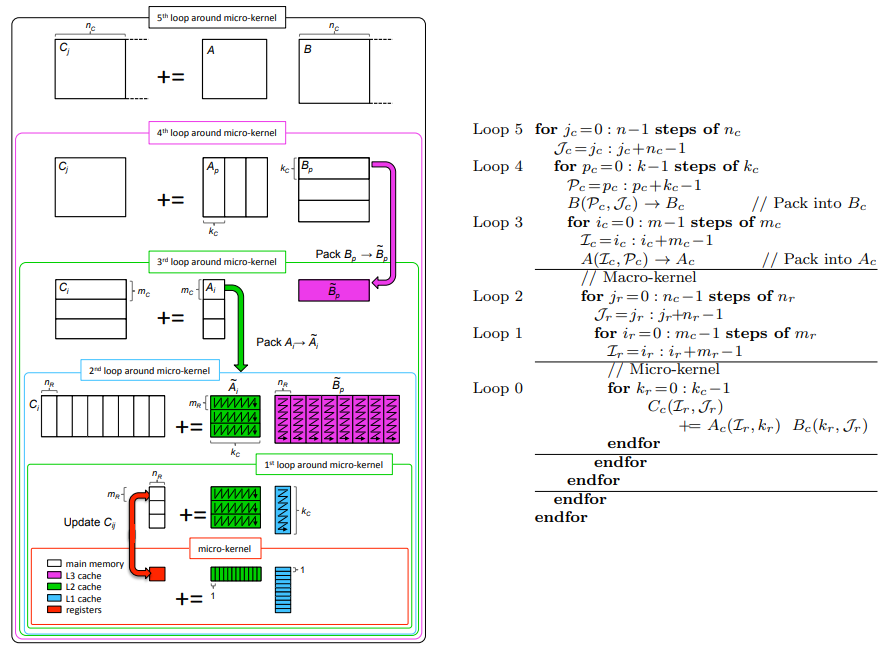
\includegraphics[width=1\textwidth]{appendices/blas.png}
\caption{Schematic Blueprint of the OpenBlas approach}
\label{fig:blas}
\end{figure}

\subsubsection{Memory Packing (Macro-Kernel Logic)}
The foundation of this architecture is the deliberate reorganization of the working set into perfectly contiguous memory buffers before any math is performed. Instead of reading directly from the global row-major matrices during the arithmetic operations, the outer loops (often called the ``macro-kernel'') extract sub-matrices and pack them into custom linear arrays.

\begin{itemize}
    \item \textbf{Packing Matrix B (L3 Cache):} Matrix $B$ is traversed in large blocks. Because $B$ is stored in row-major order, reading down its columns during a standard multiplication is highly inefficient (because of the cache-eviction due to the k-way associativity).
    
    The packing routine copies these elements into a tightly packed, sequential buffer: this reorganizes the data so that the specific elements needed simultaneously by the inner hardware are strictly adjacent in memory. This large packed block is designed to persist comfortably in the CPU's massive L3 cache.
    
    \item \textbf{Packing Matrix A (L2 Cache):} Similarly, matrix $A$ is processed in specific blocks: the packing function reshapes these blocks into smaller, contiguous micro-panels perfectly sized to remain resident in the ultra-fast L2 cache without risking eviction.
\end{itemize}

A due observation is that despite the overhead caused by the copying of the blocks elsewhere, this approach allows for a erformance gain very tangible, since now the cache can be perfectly exploited without any eviction.

\subsubsection{Micro-Kernel} 
Once the data is safely stored in contiguous cache regions (the just allocated blocks), the computation is handed off to the micro-kernel: a function computes a tiny, fixed-size spatial block (such as a $4\times8$ grid, in our implementation) of the resulting matrix $C$. 

Instead of constantly fetching and saving intermediate sums to the L1 cache, the micro-kernel operates entirely  within the CPU's vector registers. 

The exact implementation is defined in Listing~\ref{blas_like_code}:
\begin{itemize}
    \item The CPU allocates a dedicated set of vector registers to act as permanent accumulators for the small $C$ sub-block being calculated.
    \item During the accumulation loop, contiguous chunks of data from the packed $B$ and $A$ panels are loaded directly into the remaining registers.
    \item Because the data was pre-packed, these memory loads are perfectly sequential, allowing the hardware to perform simultaneous multiply-add operations at maximum theoretical throughput.
    \item Only after the entire deep accumulation loop finishes does the micro-kernel write the final computed values back to the unaligned, row-major destination matrix $C$ in global memory. 
\end{itemize}

By strictly keeping the active math inside the vector registers and the active data inside perfectly sized, sequential cache buffers, this architecture virtually eliminates memory bottlenecks.
\end{appendices}